\chapter{Teorie}
\section[Struční přehled amaterských družic]{Struční přehled\\ amaterských družic}

Radiokomunikace prošla ohromným vývojem v průběhu druhé polovice 20. století. Vypuštění první umělé družice Sputnik-1 v roce 1957 datujeme začátek vesmírného věku. Od té doby se otevřeli nové možnosti radioamatérův věnovat se svému koníčku, nebo výzkumu.

    Necelé čtyři roky po vypuštění první umělé družice Země se svět dočkal první amatérské umělé družice sestrojeného v rámci projektu \zkratka{OSCAR} \cite{wiki:amateur_sat}, kterého nástupnickou organizaci se stal \zkratka{AMSAT} \cite{wiki:AMSAT}. Družice OSCAR I byla vypuštěná na nízkou oběžnou dráhu jako druhotný náklad, který vyžíval rezervy nosnosti rakety  Thor DM-21 Agena-B. Tento způsob dopravy byl zvolen z ekonomických důvodů a je dodnes používán.

    Obecně se amatérské družice nasazují na nízkou oběžnou dráhu (Low Earth Orbit -- LEO) \cite{book:ARRL_handbook}. Výhodou dráhy tohoto typu je jejich finanční nenáročnost, co je zčásti způsobená vlastností plynoucího z nazvu oběžné dráhy, výškou orbitu, který se pohybuje od $300\,\mathrm{km}$ do $2000\,\mathrm{km}$. Nedostatkem nízké oběžné dráhy je vysoká relativní rychlost družice vůči pozemní stanici, která přibližně $7{,}8\,\mathrm{\nicefrac{km}{s}}$ \cite{wiki:LEO} jehož důsledkem je rádiový signál značně postižen dopplerovským posuvem kmitočtu, kterého velikost dosahuje i $26\,\mathrm{ppm}$.



\section{Sledování a predikce pohybu těles na oběžné dráze Země}

Objekty, které se pohybují vesmírem kolem Země jsou sledovány organizacemi \cite{wiki:derbis}:
\begin{itemize}
    \item \zkratka{USSTRATCOM}(součást \zkratka{DoD})
    \item \zkratka{ESA}
    \item \zkratka{Fraunhofer-FHR}
    \item \zkratka{JPL}(součast \zkratka{NASA})
    \item \zkratka{MIT}
    \item \zkratka{EISCAT}
    \item \zkratka{USAF}
\end{itemize}

Ke sledování se používají pozemní radary, lidary, pozemní  a vesmírné teleskopy. Mezi sledované objekty patří umělé družice, pozůstatky raket a jiný vesmírný odpad. Nejrozsáhlejší katalog stavu družic udržuje Ministerstvo obrany Spojených států (\zkratka{DoD}) s názvem Space Object Catalog. Civilní varianta této databáze je provozována organizaci \zkratka{NASA}. Tyto databáze se udržují pomocí různých modelů orbitální mechaniky. Pohyby družic jsou analyticky vypočteny pomocí teorie všeobecných perturbací. Prvky dráhy této teorie jsou publikovány ve formátu \zkratka{NASA}/NORAD \zkratka{TLE}. \cite{wiki:US_space_surv}.

Proč se zabývat přesnou polohou družice? Aby jsme byly schopní provést korekci dopplerovského posuvu, musíme splnit několik požadavek výpočtu:
\begin{itemize}
%  \item přesný čas
  \item polohu pozemní stanice \footnote{pozemní stanici považujeme za stacionární vzhledem ke povrchu Země}
  \item polohu a rychlost umělé družice
\end{itemize}

%Pro korekci dopplerovského posuvu frekvence musíme znát polohu naši pozemní stanice, polohu družice a předpovědět její polohu. K tomu pozdějšímu nám právě napomáhají prvky dráhy ze souborů \zkratka{TLE} využívajíc model \zkratka{SGP4} \cite{wiki:TLE}.

\section{Výpočet rychlosti těles na oběžní dráze Země}
  Rychlost těles na oběžné dráze dráze lze precizně vypočítat pomocí vztahu \cite{wiki:orb_speed}:

  \begin{equation}
    v = \sqrt{\mu - \left( \frac{2}{r} - \frac{1}{a} \right)}
  \end{equation}

  kde $\mu$ je standardní gravitační parametr, $v$ je rychlost tělesa, $r$ je vzdálenost tělesa od místa pozorování, $a$ je délka hlavní poloosy.

  \begin{table}[ht]
    \begin{tabular}{l | c c }
      orbita        & výška orbitu     & rychlost orbitu                        \\
      $[-]$         & $[\mathrm{km}]$  & $[\nicefrac{\mathrm{km}}{\mathrm{s}}]$ \\
      \hline
      LEO           & $200$ -- $2000$  & $6{,}9$ -- $7{,}8$ pro kruhovou dráhu  \\
      Molnija       & $500$ -- $39900$ & $6{,}5$ -- $8{,}2$ pro eliptickou dráhu\\
      Geostacinární & $35768$          & $0{,}97$ -- $1{,}08$
    \end{tabular}
    \caption{Tangenciální rychlost pro různé orbity \cite{wiki:orb_speed}}
  \end{table}

\section{Určení dopplerovského posuvu}
  Pozorovatel, který je v relativním pohybu vzhledem ke zdroji vlnění, bude vnímat vlnění se změněným kmitočtem. V případě, že relativní rychlost se mění časem, mění se i velikost změny kmitočtu. Tuto změnu kmitočtu nazýváme dopplerovským posuvem a jev se nazývá Dopplerův jev, který byl publikovaný Christianem Dopplerem v roce 1842 v Praze.

  Velikost dopplerovského posuvu lze přibližně určit pomocí vztahu \cite{wiki:doppler_effect}:
  \begin{equation}
    \Delta f = \frac{\Delta v}{c} f_0
  \end{equation}

  kde $\Delta f$ je posuv kmitočtu, $\Delta v$ je relativní rychlost, $c$ rychlost vln v prostředí, $f_0$ je původní kmitočet.

  Pro výpočet dopplerovského posuvu signálu vysílaného družicí na oběžné dráze Země je potřebné znát její relativní rychlost vzhledem k pozorovateli na pozemní stanici. Tuto rychlost lze vypočítat z oběžné rychlosti družice pomocí trigonometrických výpočtů. Princip je zobrazen na obrázku \ref{img:rel_vel}
  \begin{figure}[ht]
    \centering
    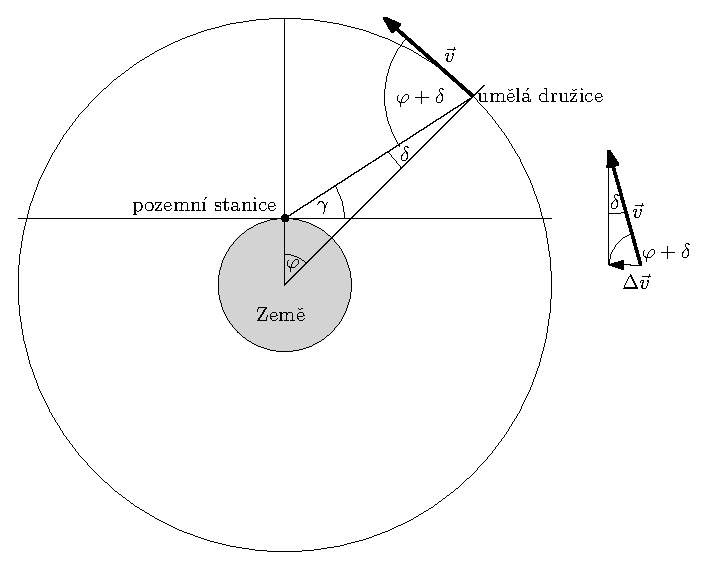
\includegraphics{./obrazky/doppler_shift.eps}
    \caption{Výpočet vektoru relatívní rychlosti \cite{book:doppler_compensation}}
    \label{img:rel_vel}
  \end{figure}


%\chapter{Korekce dopplerovského posuvu}
%  TBD\dots
%
%\chapter{Demodulace a dekódování signálu}
%  TBD\dots
